\section{Experiment Execution}
\subsection{Experiment Setup}
This section elaborates on the technical specifications of the infrastructure including software applications and hardware devices we use to execute the experiment. 

	Figure 2 illustrates the experimental setup that constitutes two core components, they are: (1) an Android device for running two music streaming applications, and (2) the Raspberry Pi for configuring and conducting the experiment as well as collecting the data. The Android device and the Raspberry Pi are connected via USB. Communication between them is achieved by a command-line tool Android Debug Bridge (adb)\footnote{\label{note1}\href{ https://developer.android.com/studio/command-line/adb }{https://developer.android.com/studio/command-line/adb}}. 

\begin{figure}[htbp]
 \centering
 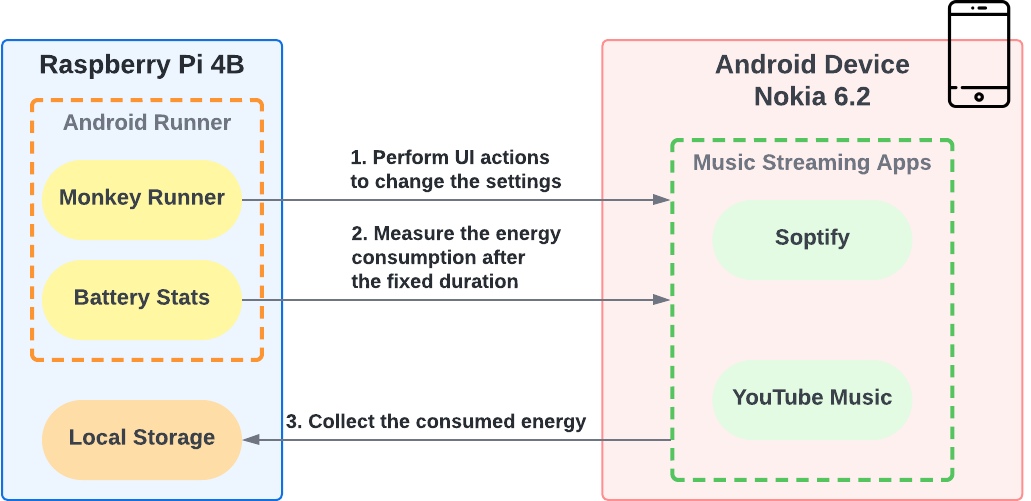
\includegraphics[width=0.8\linewidth]{figures/workflow.png}\textcolor{blue}{\caption{Experiment workflow and infrastructure}}
\end{figure}

Two music streaming applications Spotify (version 8.7.68.568, released on 22.09.2022) and YouTube Music (version 5.25.51, released on 22.09.2022) are installed from Google Play store, and run on the Nokia 6.2 mobile phone. {\color{blue}Table 4 and Table 5 report the technical specifications of Nokia 6.2 and Raspberry Pi 4B in detail, respectively.}

Special care is taken to mitigate the effect that irrelevant factors may pose on the outcome, especially network and execution environment. On the one hand, both devices run under the same Wi-Fi network and are placed at the same distance from the router. Besides, they are the only devices that are connected to the network (if needed) during the experiment. On the other hand, the Android device is prohibited from OS updates and all third-party applications are uninstalled. 

\begin{table}[t]
\centering
\caption{Nokia 6.2 - technical specifications}
\label{table1}
\begin{tabular}{|c|c|}
\hline
CPU & 1.8 GHz Qualcomm Kryo 260 Octa-core\\
\hline

Memory & 4GB \\ 
\hline

Disk space &  64GB \\
\hline

Battery capacity &  3500 mAh \\
\hline

Screen &  6.3 inch, FHD+ \\
\hline

OS & Android 10.0 \\
\hline

\end{tabular}
\label{table_MAP}
\end{table}

\begin{table}[t]
\centering
\caption{{\color{blue}Raspberry Pi 4B - technical specifications}}
\label{table1}
\begin{tabular}{|c|c|}
\hline
{\color{blue}CPU} & {\color{blue}1.5 GHz Quad-Core 64-bit Arm Cortex A72}\\
\hline

{\color{blue}Memory} & {\color{blue}2GB} \\ 
\hline

{\color{blue}Disk space} &  {\color{blue}4GB} \\
\hline

{\color{blue}Power Supply} &  {\color{blue}18W 5V 3.6A Power Supply} \\
\hline

{\color{blue}OS} &  {\color{blue}Ubuntu 20.04} \\
\hline


\end{tabular}
\label{table_MAP}
\end{table}

In order to automate the experiment, we take advantage of the Python framework Android Runner\footnote{\label{note1}\href{ https://github.com/S2-group/android-runner }{https://github.com/S2-group/android-runner}}. We leverage an Android testing tool MonkeyRunner\footnote{\label{note1}\href{ https://developer.android.com/studio/test/monkeyrunner  }{https://developer.android.com/studio/test/monkeyrunner }} to have full control over the experiment execution. Specifically, Monkeyrunner is able to record a sequence of UI events and then replay them per request. In accordance with Android Runner, the experiment configuration is documented in JSON files that instruct Android Runner to run the experiment. Additionally, among all plugins that are integrated into Android Runner, we utilize Batterystats\footnote{\label{note1}\href{ https://github.com/S2-group/android-runner/tree/master/AndroidRunner/Plugins/batterystats}{\url{https://github.com/S2-group/android-runner/tree/master/AndroidRunner/Plugins/batterystats}}} to estimate the energy consumption in each run. {\color{blue}Batterystats is a plugin included in the Android framework that can be integrated into adb to dump the collected battery statistics to the working machine. }

All statistical tests are performed on RStudio\footnote{\label{note1}\href{ https://www.rstudio.com/products/rstudio/download/    }{https://www.rstudio.com/products/rstudio/download/ }} (version 4.1.2 released on 11.2021). R packages ggplot2\footnote{\label{note1}\href{ https://ggplot2.tidyverse.org/   }{https://ggplot2.tidyverse.org/}} is used for data visualization whereas effectsize\footnote{\label{note1}\href{  https://cran.r-project.org/web/packages/effectsize/index.html    }{ https://cran.r-project.org/web/packages/effectsize/index.html }} is for calculating the effect size. 

\subsection{Experiment Workflow}
To begin with, the Python script is executed to initialize an instance of Android Runner that is related to the corresponding configuration file. During one run, each instance launches the application, and sequentially alters the settings to match the current treatment parameters. Next, the Batterystats profiler comes into play. It records the energy consumption during the three minutes trial, after which Android Runner shuts down the application, followed by a one minute cooldown period. 

Precautions are taken to reduce the intrinsic variability of energy measurement. First of all, each measurement is applied 30 times. Secondly, the execution order of each treatment is randomized. Plus, a one minute idle time is added between each run to avoid tail energy usage where certain hardware components are kept active by the operating system to lower startup energy costs \cite{li2013calculating}. Finally, cache is cleared before each run to enforce the streaming in the Wi-Fi environment. 

\href{https://docs.google.com/spreadsheets/d/1w2QG47_3Y9-IXbPPSM2fw1bH0ZvWMfadzRdfwqmWBtI/edit?usp=sharing}{\textbf{Time Log}}


